\documentclass[
% table,
% compress,
% usenames,
% dvipsnames,
% aspectratio=169,
9pt, % font size
% draft, % consider using this for speed
 handout, % remove the overlays
% t, % place stuff at the top instead of at the center
]{beamer}
\usepackage{import}
\usepackage{graphicx}
% beamer theme
\usetheme{Luebeck}
\useinnertheme{circles}
\usecolortheme{simula} % Simula UiB colors
\usefonttheme[onlymath]{serif} % standard LaTeX font for math
\usefonttheme{sourcepro} % Simula UiB fonts

% font theme
\setbeamerfont{title}{size=\huge,series=\bfseries,parent=structure}
\setbeamerfont{block body}{}
\setbeamerfont{block body alerted}{}
\setbeamerfont{block body example}{}
\setbeamerfont{block title}{size=\large,parent={structure,block body}}
\setbeamerfont{block title alerted}{parent={block title,alerted text}}
\setbeamerfont{block title example}{parent={block title,example text}}

% itemize font
% \setbeamerfont{item}{parent=structure}
% \setbeamerfont{subitem}{parent=item}
% \setbeamerfont{subsubitem}{parent=subitem}

% \setbeamerfont{item projected}{size=\tiny,parent={item,projected text}}
% \setbeamerfont{subitem projected}{parent=item projected}
% \setbeamerfont{subsubitem projected}{parent=subitem projected}

% \setbeamerfont{itemize item}{parent=item}
% \setbeamerfont{itemize subitem}{parent=subitem}
% \setbeamerfont{itemize subsubitem}{parent=subsubitem}

% \setbeamerfont{enumerate item}{parent=item}
% \setbeamerfont{enumerate subitem}{parent=subitem}
% \setbeamerfont{enumerate subsubitem}{parent=subsubitem}

% \setbeamerfont{itemize/enumerate body}{}
% \setbeamerfont{itemize/enumerate subbody}{size=\small}
% \setbeamerfont{itemize/enumerate subsubbody}{size=\footnotesize}

% define footer
\setbeamertemplate{footline}
{%
  \leavevmode%
  \hbox{%
    \begin{beamercolorbox}[wd=.12\paperwidth,ht=2.5ex,dp=1.125ex,leftskip=.2cm
      plus1fill,center] {author in head/foot}%
      \usebeamerfont{author in head/foot} \insertframenumber{} / \inserttotalframenumber
    \end{beamercolorbox}%
    \begin{beamercolorbox}[wd=.23\paperwidth,ht=2.5ex,dp=1.125ex,leftskip=.3cm,rightskip=.3cm plus1fil]{author in head/foot}%
      \usebeamerfont{author in head/foot}\insertshorttitle
    \end{beamercolorbox}}%
    \begin{beamercolorbox}[wd=.45\paperwidth,ht=2.5ex,dp=1.125ex,leftskip=.3cm,
      rightskip=.3cm]{author in head/foot}%
      \usebeamerfont{author in head/foot}\insertshortauthor
    \end{beamercolorbox}%
    \begin{beamercolorbox}[wd=.2\paperwidth,ht=2.5ex,dp=1.125ex,right,rightskip=.2cm]{section in head/foot}%
      \hspace*{2ex} 
      {%
        \vspace*{-1mm}%
        
\includegraphics[scale=0.04, trim=0 -2cm 0 0]{./theme_figures/pdf/Emblem_blaa.pdf}%
      }%
    \end{beamercolorbox}
  \vskip0pt%
}

% define header
\setbeamertemplate{headline}{}

% make covered text faded instead of invisible
\setbeamercovered{invisible}

% disable mouse navigation bar
\beamertemplatenavigationsymbolsempty

% add packages here
\usepackage{pgfpages}
\usepackage{graphicx}
\usepackage{graphics}
\usepackage{setspace}
\usepackage{color}
\usepackage{colortbl}
\usepackage{multirow}
\usepackage{array}
\usepackage{xspace}
\usepackage{tikz}
\usepackage{pgfplots}
\usepackage[absolute,overlay]{textpos}
\usepackage{ctable}
\usepackage{mathtools}
\usepackage{pbox}
\usepackage[export]{adjustbox}
\usepackage{amsmath} % improved math formulas
\usepackage{amssymb} % math symbols
\usepackage{amsthm} % theorem environments
\usepackage{thmtools} % extends amsthm with autoref compat. etc.
\usepackage{bm} % bold math
\usepackage{csquotes} % context-sensitive quotation
\usepackage{balance} % balance columns on the final page
\usepackage{cite} % sorted references etc.
\usepackage{addlines} % add/remove lines from length of a page
\usepackage[square]{natbib} % use separate citation and bibliography styles
\usepackage[normalem]{ulem}
\usepackage{comment}


% add macros here

% print references in the ieee style and references like Author et al. (year)
\bibliographystyle{IEEEtranN}
\setcitestyle{apalike}

% setup title frame
\title[Main module]{Main Module of the Project}
\author[A. Severinson]{Albin~Severinson}
\institute[Simula UiB]{
  \normalsize{Simula UiB, Bergen, Norway}

  \vspace*{5mm}{
    
\includegraphics[width=0.4\textwidth]{../theme_figures/pdf/MainLogo_Blaa.pdf}
  }\vspace*{5mm}
}
\date{
Beamer Template\\
~\\September 14, 2020
}

\iffalse
\AtBeginSection[]
{
  \begin{frame}<beamer>[plain]
    \frametitle{Outline}
    \tableofcontents[currentsection]
  \end{frame}
}
\fi

\begin{document}

% title frame
\begin{frame}[plain, c, noframenumbering]
  \begin{center}
    \titlepage
  \end{center}
\end{frame}

\begin{frame}
  \frametitle{Frame title}
  \center \Huge Main module content

  \vspace{2cm}
  \normalsize%
  Reference:~\cite{Severinson2018tcom}
\end{frame}

\begin{frame}
  \begin{figure}
    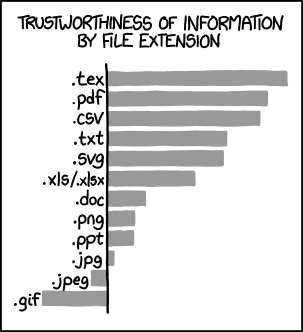
\includegraphics[width=0.5\textwidth]{../Figures/file_extensions.png}
    \caption{Figure include from main.tex}
  \end{figure}
\end{frame}

\begin{frame}
  \frametitle{Tikz figure include from main.tex}

  \begin{figure}
    \documentclass[tikz,9pt]{standalone}

% add packages here
\usepackage{pgfpages}
\usepackage{graphicx}
\usepackage{graphics}
\usepackage{setspace}
\usepackage{color}
\usepackage{colortbl}
\usepackage{multirow}
\usepackage{array}
\usepackage{xspace}
\usepackage{tikz}
\usepackage{pgfplots}
\usepackage[absolute,overlay]{textpos}
\usepackage{ctable}
\usepackage{mathtools}
\usepackage{pbox}
\usepackage[export]{adjustbox}
\usepackage{amsmath} % improved math formulas
\usepackage{amssymb} % math symbols
\usepackage{amsthm} % theorem environments
\usepackage{thmtools} % extends amsthm with autoref compat. etc.
\usepackage{bm} % bold math
\usepackage{csquotes} % context-sensitive quotation
\usepackage{balance} % balance columns on the final page
\usepackage{cite} % sorted references etc.
\usepackage{addlines} % add/remove lines from length of a page
\usepackage[square]{natbib} % use separate citation and bibliography styles
\usepackage[normalem]{ulem}
\usepackage{comment}


% add macros here

\begin{document}

\begin{tikzpicture}
\node [] at (0,0) (simulablue) {
\includegraphics[width=2cm]{../theme_figures/pdf/MainLogo_Blaa.pdf}};

\node [] at (3,0) (simulablack) {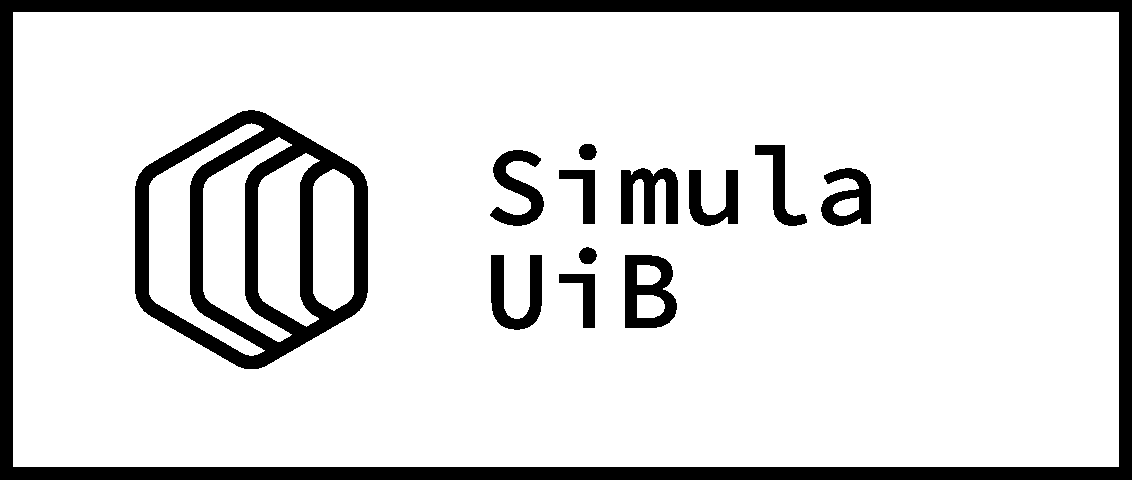
\includegraphics[width=2cm]{../theme_figures/pdf/MainLogo_sort.pdf}};
\end{tikzpicture}

\end{document}
  \end{figure}
\end{frame}

% Import the submodule
\subimport{../Submodule}{submodule.tex}

\begin{frame}[t,allowframebreaks]
  \frametitle{References}
  \tiny{\bibliography{../manuscript}}
\end{frame}

\end{document}
